\chapter{Link Prediction}

\section{Algorithmen}
Link-Predictions basieren auf einem bestehenden Netzwerk und versuchen, neue Kanten hervorzusagen.
Es gibt verschiedene Algorithmen, um diese Kanten vorherzusagen.
Initial werden im Plugin die Algorithmen ``Common Neighbours'' und ``Preferential Attachment'' implementiert. Diese werden nachfolgend genauer beschrieben.

Die Funktionsweise der besagten Algorithmen wird anhand von konkreten Beispielen veranschaulicht.
Als Grundlage für die Vorhersagen wird der Beispielgraph aus Abbildung \ref{fig:graph_bsp} verwendet.

\begin{figure}[h]
    \centering
    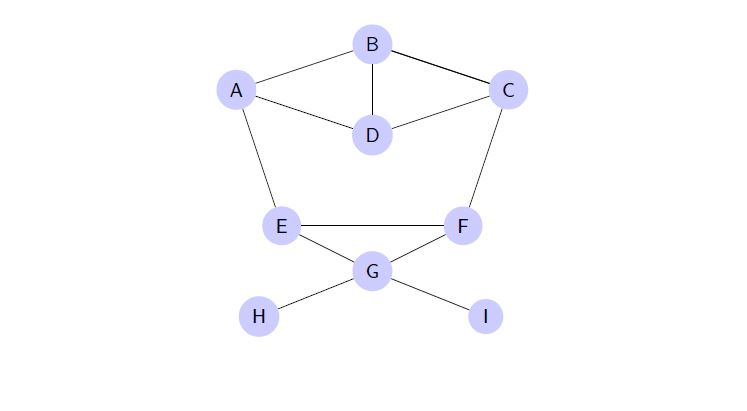
\includegraphics[scale=0.7]{resources/graph_example.JPG}
    \caption{Beispielgraph}
    % TODO Add cite to SNA Script
    \label{fig:graph_bsp}
\end{figure}

\subsection{Common Neighbours}
Der Common Neighbours Algorithmus berechnet für zwei nicht verbundene Knoten, wie viele gemeinsame Nachbarn existieren. Die Wahrscheinlichkeit
für das Entstehen einer neuen Kante ist umso höher, desto mehr gemeinsame Nachbarn zwei
Knoten haben. Common Neighbours beruht auf dem Social Forces Prinzip der Homophilie: Je grösser die Anzahl Gemeinsamkeiten in Form von Nachbarn, desto wahrscheinlicher wird eine neue Kante zwischen den beiden Knoten hinzugefügt (vgl. Kapitel \ref{socialforces}).

Die folgende Formel zeigt, wie die Anzahl der gemeinsamen Nachbarn von zwei Knoten $X$ und $Y$ berechnet werden kann::

\begin{equation}
\label{eq:cn}
    common\_neighbours(X,Y) = | N(X) \cap N(Y) |
\end{equation}

Der Wert, der aus der Berechnung für diesen Algorithmus resultiert, ist die Summe der Anzahl aller gemeinsamen
Nachbarn der beiden Knoten $X$ und $Y$. Dieser Wert muss für alle Knoten-Kombinationen berechnet und anschliessend der höchste
Wert ausgewählt werden.

Angewandt auf den eingangs eingeführten Beispielgraphen würde der Common Neibghour Algorithmus eine neue Kante zwischen den Nodes $A$ und $C$ vorhersagen.
Die folgenden Beispiele zeigen weitere Werte, welche durch Anwenden des Algorithmus resultieren.\\
% Layout multiline-formula
\\
\vspace{4mm}
% Set identiation manually
\newcommand{\forceindent}{\leavevmode{\parindent=2em\indent}}
\forceindent $common\_neighbours(A,C) = |{B, D}| = 2$\\
\vspace{4mm}
\forceindent $common\_neighbours(A,F) = |{E}| = 1$\\
\vspace{4mm}
\forceindent $common\_neighbours(A,I) = |{\{\}}| = 0$\\

Das Code-Listing \ref{lstCommonNeighbour} zeigt die vereinfachte Implementierung des Algorithmus.
Weil initial zweimal über sämtliche Knoten iteriert werden muss, besitzt die Implementierung die Komplexitätsklasse $O(n^2)$.

%TODO: Make sure naming e.g. calculate is correct
\begin{lstlisting}[caption={Common neighbour implementation},label=lstCommonNeighbour]
    // CommonNeighboursStatistics.java
    public void calculateAll(Graph graph) {

        //Iterate over all nodes
        for (Node a : graph.getNodes()) {

            // Remove self from nodes,
            // of which neighbourhood will be
            // verified
            List<Node> others = graph.getNodes().remove(a);

            // Get neighbours of a
            List<Node> aNeighbours = getNeighbours(graph, a);

            //Calculate common neighbours
            for (Node b : others) {

                // Get neighbours of b
                List<Node> bNeighbours = getNeighbours(graph, b);
                // Count number of common neighbours
                int commonNeighboursCount = getCommonNeighboursCount(aNeighbours, bNeighbours);

                // Temporary save calculated
                // value if edge does not exist
                if (isNewEdge()) {
                    saveCalculatedValue(a, b, commonNeighboursCount)
                }
            }
        }

        // Add edge with highest calculation to graph
        Edge max = getHighestPrediction();
        graph.addEdge(max, "Common Neighbours);

    }
\end{lstlisting}

\subsection{Preferential Attachment}
Mit dem Preferential Attachment Algorithmus werden ebenfalls die Nachbarn eines Knotens berücksichtigt. Diese müssen jedoch nicht
mit den Nachbarn des anderen Knoten übereinstimmen - es geht lediglich um die Anzahl der eigenen Nachbarn. Bei Preferential Attachment
wird von der Annahme ausgegangen, dass die Wahrscheinlichkeit einen neuen Kontakt zu knüpfen grösser wird, je grösser das eigene Netzwerk bereits ist.
Die Entstehung eines neuen Edges wird in diesem Fall nicht über Homophilie bestimmt, sondern über Ansehen (vgl. Kapitel \ref{socialforces}).

Die Formel für den Preferential Attachment Algorithmus lautet wie folgt:

\begin{equation}
    \label{eq:pa}
    preferential\_attachment(X,Y) = | N(X) | \cdot | N(Y ) |
\end{equation}

Um den resulierenden Wert zu erhalten, wie die Anzahl Nachbarn zweier Knoten $X$ und $Y$ miteinander multipliziert. Dieser Wert muss für alle Knoten-Kombinationen berechnet und anschliessend der höchste Wert
ausgewählt werden.

Angewandt auf den Beispielgraphen würde mit Preferential Attachment eine Kante zwischen den Knoten $A$ und $G$ vourausgesagt und folgende weiteren Werte berechnet:\\
% Layout multiline-formula
\\
\vspace{4mm}
% Set identiation manually
\forceindent $preferential\_attachment(A,G) = 3 * 4 = 12$\\
\vspace{4mm}
\forceindent $preferential\_attachment(A,C) = 3 * 3 = 9$\\

Das Code-Listing \ref{lstPreferentialAttachment} zeigt die vereinfachte Implementierung des Algorithmus. Der Algorithmus besitzt die Komplexitätsklasse $O(n^2)$.

\begin{lstlisting}[caption={Preferential attachment implementation},label=lstPreferentialAttachment]
    // PreferentialAttachmentStatistics.java
    public void calculateAll(Graph graph) {

        //Iterate over all nodes
        for (Node a : graph.getNodes()) {

            // Remove self from nodes,
            // of which neighbourhood will be
            // verified
            List<Node> others = graph.getNodes().remove(a);

            // Get neighbours of a
            List<Node> aNeighbours = getNeighbours(graph, a);

            //Calculate preferential attachment
            for (Node b : others) {

                // Get neighbours of b
                List<Node> bNeighbours = getNeighbours(graph, b);
                // Multiply number of neighbours
                int totalNeighboursCount = aNeighbours.size() * bNeighbours.size();

                // Temporary save calculated
                // value if edge does not exist
                if (isNewEdge()) {
                    saveCalculatedValue(a, b, totalNeighboursCount)
                }
            }
        }

        // Add edge with highest calculation to graph
        Edge max = getHighestPrediction();
        graph.addEdge(max, "Preferential Attachment");

    }
\end{lstlisting}

\section{Evaluation}
Basierend auf zwei Graphen wird die Genauigkeit der Vorhersagen unter Verwendung verschiedener Algorithmen bewertet.
Ausgehend von einem initialen Graphen $G_i_,_t$ zum Zeitpunkt $t$ prognostizieren wir $n$ Kanten $E_i$, was zu einem Graphen $G_i_,_t_+_n$ zum Zeitpunkt $t + n$ führt.
Dieser neue Graph $G_i_,_t_+_n$  wird zur Validierung der vorhergesagten Kanten verwendet.
Abbildung \ref{fig:graph_init} zeigt die Graphen $G_i_,_t$ (links) und $G_i_,_t_+_n$ (rechts) anhand des vorhin eingeführten Beispiels.
Die hinzugefügten Kanten $E_i$ sind dabei mit einer gestrichelten Linie eingezeichnet.

\begin{figure}[h]
    \centering
    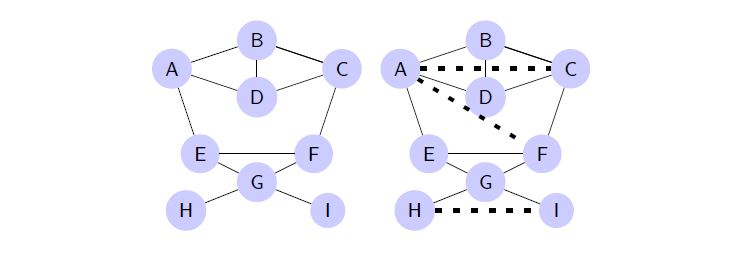
\includegraphics{resources/graph_init.JPG}
    \caption{Initialer Graph zum Zeitpunkt $t$, resp. $t + n$}
    % TODO Add cite to SNA Script
    \label{fig:graph_init}
\end{figure}

Die Qualität des Algorithmus wird anhand der Genauigkeit der hinzugefügten Kanten bestimmt.
Dazu wird ein Validierungsgraph $G_v_,_t_+_n$ verwendet, bei welchem die zusätzlichen Kanten $E_v$ zum Zeitpunkt $t + n$ bereits vorhanden sind.
In unserem Beispielnetzwerk enthält dieser Graph gegenüber dem Graphen $G_i_,_t$ zusätzlich die Kanten $(A,C)$, $(E,H)$ und $(H,I)$.
Abbildung \ref{fig:graph_validation} zeigt den Graphen $G_v_,_t_+_n$ zum Zeitpunkt $t + n$

\begin{figure}[h]
    \centering
    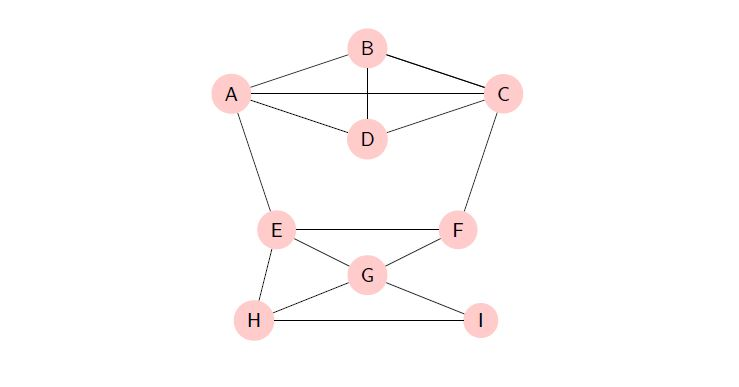
\includegraphics{resources/graph_validation.JPG}
    \caption{Validierungsgraph zum Zeitpunkt $t + n$}
    % TODO Add cite to SNA Script
    \label{fig:graph_validation}
\end{figure}

Als Qualitätsmass wird die Accuracy verwendet.
Diese berechnet sich als prozentualer Anteil der korrekt vorhergesagten Kanten im Verhältnis zu allen hinzugefügten Kanten.

\begin{equation}
    \label{eq:acc}
    Acc = | E_i \ \cap \ E_v| \ / \ |E_v| * 100
\end{equation}

Im obigen Beispiel mit drei zusätzlichen Kanten wurden die Kanten $(A,C)$ und $(H,I)$ korrekt vorhergesagt.
Daraus folgt eine Accuracy von 66.67\%.
Die Herleitung dazu sieht folgendermassen aus:\\
% Layout multiline-formula
\\
\vspace{4mm}
\forceindent $E_i = \{(A,C), (A,F), (H,I)\}$\\
\vspace{4mm}
\forceindent $E_v = \{(A,C), (E,H), (H,I)\}$\\
\vspace{4mm}
\forceindent $| E_i \ \cap \ E_v| = |\{(A,C), (H,I)\}| = 2$\\
\vspace{4mm}
\forceindent $Acc = | E_i \ \cap \ E_v| \ / \ |E_v| * 100 = 2 \ / \ 3 * 100 = 66.67$\\
% TODO: Performance-Optimierung hier schon erwähnen?

\section{Gegenüberstellung der verschiedenen Algorithmen und Netzwerke}
Die Qualität der verschiedenen Algorithmen kann beurteilt werden, indem die eben eingeführte Accuracy auf die Daten aus Kapitel \ref{daten} angewendet wird.
Um die Qualität der Algorithmen besser beurteilen zu können, wird die Entwicklung mit zunehmender Anzahl Iterationen betrachtet.
In jedem Iterationsschritt wird eine neue Kante zu den Graphen hinzugefügt und die Accuracy zu diesem Zeitpunkt berechnet.

Die Tabelle \ref{tab_accuracy_iter} zeigt die Accuracy für die verschiedenen Datensets nach 1, 10, 50 und 100 Iterationen.

\begin{table}[]
    \centering
    \resizebox{\textwidth}{!}{%
    \begin{tabular}{@{}llrll@{}}
        \toprule
        Datenset                         &          & \multicolumn{1}{l}{10} & 50       & 100      \\ \midrule
        Les Miserables                   & 0.000234 & 0.000234               & 0.000234 & 0.000234 \\
        Coauthorships in network science & 0.000234 & 0.000234               & 0.000234 & 0.000234 \\
        Power grid                       & 0.000234 & 0.000234               & 0.000234 & 0.000234 \\ \bottomrule
    \end{tabular}%
    }
    \caption{Metrikwerte der Netzwerke}
    \label{tab_accuracy_iter}
    %TODO Add correct values to table
\end{table}
